\chapter{Einleitung}\label{Einleitung}
In Forschungseinrichtungen und in Unternehmen arbeiten viele Menschen mit unterschiedlichen Aufgaben und Tätigkeiten.
Manche wissen jedoch nichts darüber was andere Mitarbeiter machen, wenn sie nicht direkt mit ihnen zusammen arbeiten.
Einige Mitarbeiter wollen ihre Kollegen oder Gäste über ihre aktuelle Arbeit, wichtige Termine oder kommende Veranstaltungen informieren.
Andere möchten gern den Inhalt ihrer letzten wissenschaftlichen Ausarbeitung, die Ergebnisse der letzten Konferenz, Noten einer bestimmten Prüfung oder einfach nur private Daten präsentieren.
Um diese Informationen zur Verfügung zu stellen werden in den meisten Büros Pinnwände oder Whiteboards neben den Türen aufgehangen \abb{img:pinnwand}. Um kurze Nachrichten zu hinterlassen, kleben einige Personen Post-Its an ihre Tür oder hängen ``Do-Not-Disturb''-Schilder an den Türknauf, wenn sie nicht gestört werden wollen.
\\
\begin{figure}[h!]
  \centering
  %\captionsetup{justification=centering}
    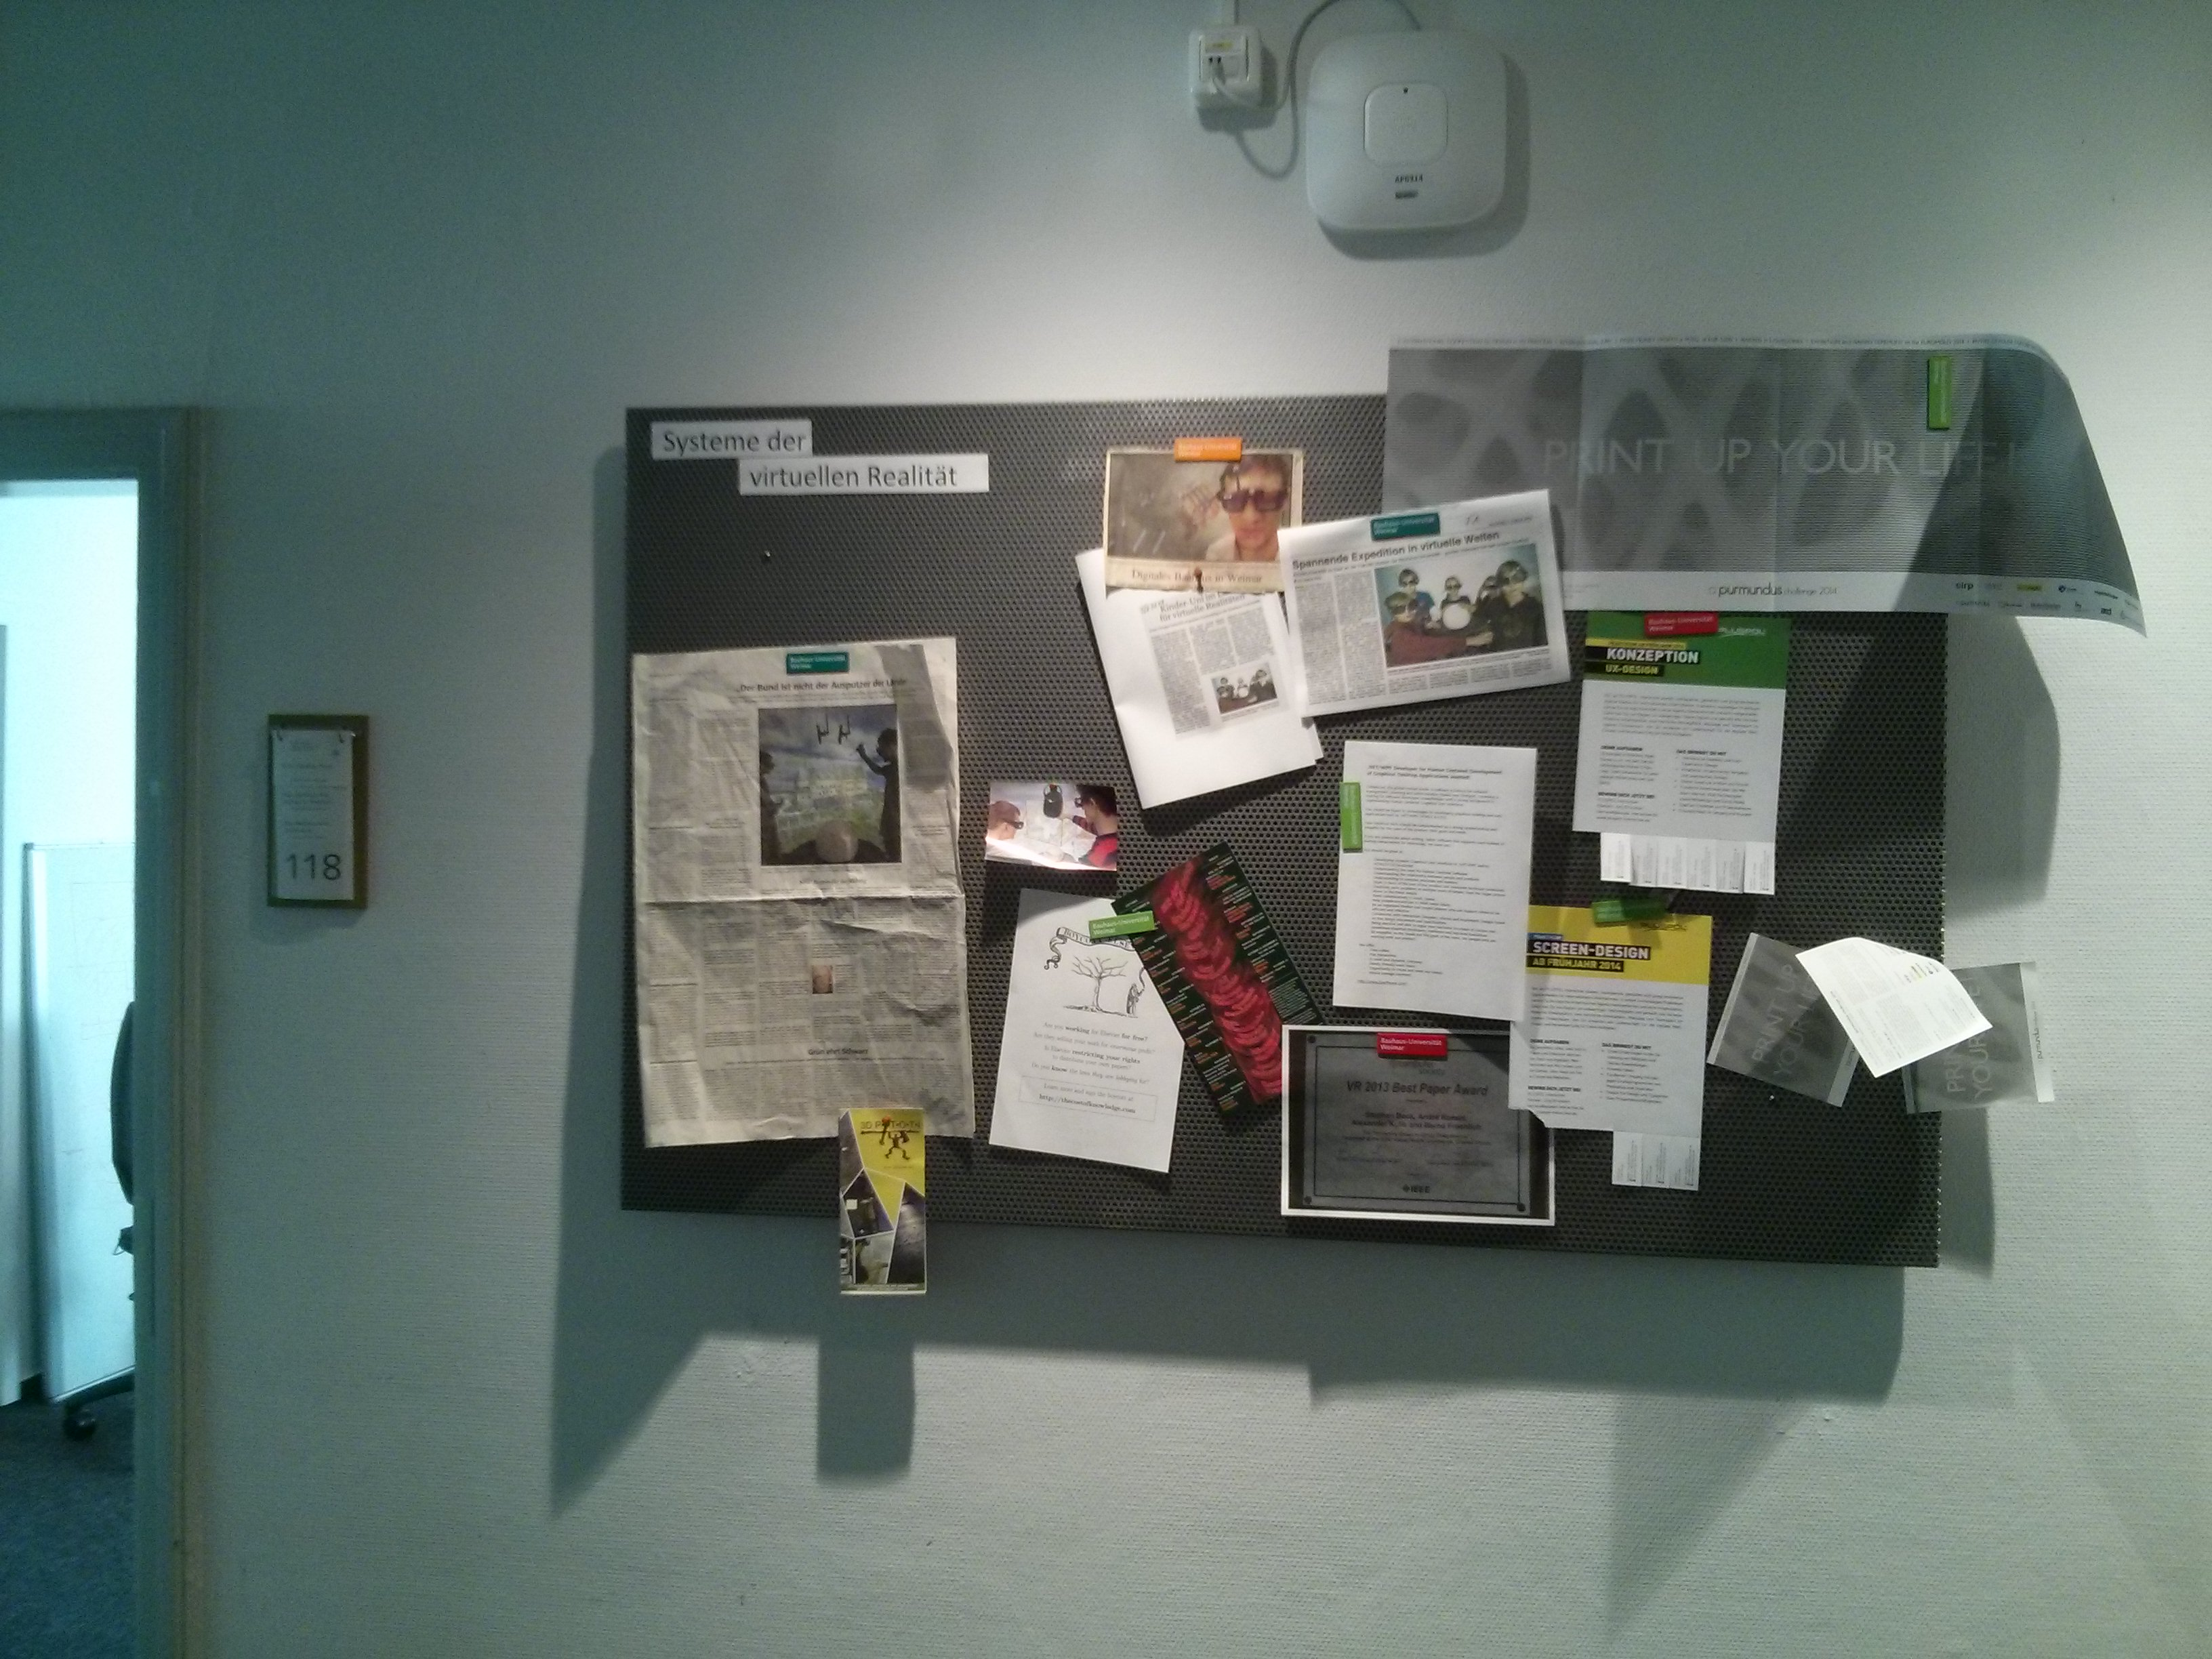
\includegraphics[width=0.6\textwidth]{./img/pinnwand.jpg}
  \caption{Typische Pinnwand der Medienfakultät der BUW}
  \label{img:pinnwand}
\end{figure}
\\
Aktuell müssen die Personen des Raumes solche Informationen direkt an die Wand schreiben oder ausdrucken und danach dort aufhängen.
Wenn man aber nicht persönlich vor Ort ist, kann man die Daten an der eigenen Pinnwand nicht selbst anpassen.
Es kann zu Problemen kommen, wenn man zum Beispiel einen Termin vereinbart hat und sich dann verspätet, wenn man krank geworden ist und deswegen den ganzen Tag nicht anzutreffen ist oder auf einer Reise ist und andere am Arbeitsplatz direkt daran teilhaben lassen möchte.
\\
Pinnwände und Whiteboards bieten zudem auch nicht die Möglichkeit digitale Informationen, wie Videos, animierte Gifs\footnote{Ein Gif (Graphic Interchange Format) ist ein Grafikformat mit dem mehrere Bilder in einer Datei gespeichert und von Webbrowsern als Animation interpretiert werden können.} oder die neuesten Twittermeldungen anzuzeigen.
\\
Eine Lösung für diese Probleme ist die Anbringung eines digitalen Türschildes, mit welchem Nutzer direkt oder aus der Ferne interagieren können.
\\
\\
Zu Beginn galt es zu klären, welchen Weg ich mit dieser Arbeit einschlagen sollte.
\todotext{zum einen ohne zum anderen, vllt Entweder?}\\
\todotext{hernehmen, anderes wort}
Zum einen konnte ich ein bereits vorhandenes Projekt hernehmen, anpassen und verbessern oder ein eigenes System von Grund auf selbst entwerfen und umsetzen.
Deshalb führte ich ein Experiment mit dem NetBoards System\cite{wood:2014,netboards:website} durch, um herauszufinden, ob dies ein geeignetes System für die Verwendung an der Medienfakultät der BUW wäre. Zudem ging es darum die Bedürfnisse und das Verhalten der Benutzer im Bezug zu interaktiven Türschildern zu ermitteln.
\\
Nach der Durchführung des Experimentes stellte sich heraus, dass das NetBoards System nicht der richtige Ansatz für die Umgebung war, was in Kapitel \ref{AuswertungVorstudie} erklärt wird. Deswegen entschied ich mich dazu, ein eigenes System zu entwerfen.
\\
Die Entwicklung meines Systems teilte sich in drei Abschnitte: Planungsphase, Implementationsphase und Studienphase.
Die Planungsphase diente dazu, die Systemumgebung und den Aufbau der Applikation zu definieren.
Darunter fielen die Wahl des Anwendungstyps und der Programmiersprache sowie der Entwurf einer Datenbank und des Benutzerinterfaces.
\\
In der Implementationsphase befasste ich mich damit, die geplanten Ideen in ein lauffähiges Programm umzusetzen.
\\
Das Programm musste nach seiner Fertigstellung getestet werden. Deswegen habe ich in der letzten Phase eine Studie geplant und durchgeführt. Dafür habe ich in der Medienfakultät der BUW vor bestimmten Büros Tablets angebracht, die Interaktionen damit archiviert und im Anschluss die Testnutzer befragt. Die Ergebnisse der Befragung wurden ausgewertet und fließen in die nächste Version des Programms ein.